\chapter{Structures de données et algorithmes de base}\label{chap:moteur}
    Ici nous allons définir les règles du jeu à travers des algorithmes qui permettront d'analyser les situations probables du jeu afin de pouvoir vérifier la légalité des coups joués, ce qui nous rendra apte ensuite à créer l'IA du jeu.
    
    \section{Structure de données}
        \subsection{Goban}
            Pour l'implantation du Goban, nous avons utilisé le paradigme objet du langage C++.\\
            Avec la notion de classe qu'introduit ce dernier, on a pu définir la classe Goban pour manipuler aisément ses données par le biais des fonctions membres.\\ Le Goban se présente comme un plateau de taille 19x19, composé d'état avec ses différentes valeurs.
        \subsubsection{Accès aux états}
            Le goban est en alors un tableau d'états, dont la manipulation à l'aide des accesseurs permettent de  modifié le Goban et simulé le Jeu.
        \subsection{États}
            L'état est une représentation d'une pierre dans le plan, avec ses coordonnées et une valeur qui peut être vide, noir, blanc, KO\_Noir, KO\_Blanc, ou simplement Non jouable (NJ).
        \subsection{Territoires d'un Goban : Les groupes}
            Un Groupe est une liste d'état voisin de même valeur se trouvant dans le Goban.
            
    \section{Algorithmes} 
        \subsection{Algorithme de Recherche}
            La recherche se fait dans le Goban, en deux temps. D'abord on recherche les groupes de couleurs noirs ainsi que les groupes de couleurs blanches. Ensuite on lance la fusion sur chacun des groupes.
            La recherche de Groupe consiste à parcourir tout le Goban en largeur et vérifier si l'état courant appartient à un groupe déjà défini. Le cas échéant on rajoute la pierre à ce groupe et on passe au suivant, autrement on créer un nouveau groupe avec cette pierre.
            
            \begin{algorithme}
                \caption{RechercheGroups}
                \textbf{Données:}
                \Type{val}{VAL} ,
                \Type{Array}{Etat[]}\\
                \textbf{Résultats:} Définir les groupes de la couleur val dans Array\\
                \textbf{Variables:}
                \Type{x, i, j}{entier},
                \Type{groupe}{Groupe}
                %\textbf{Début:}
                
                x $\leftarrow$ 0\\
                \IfThenElse{val = BLANC}
                {val $\leftarrow$ groupsWhite}
                {val $\leftarrow$ groupsBlack}
                \ForFromTo{i}{0}{TGOBAN*TGOBAN}
                {
                    \If{ValArray[i] = val}
                    {
                        j $\leftarrow$ 0 \\
                        \While{j $\leq$ tailleGroups}
                        {
                            \IfThenElse{ ! (Array[i] \in groupe[j])}
                            {
                                \If{groupe[j] doitContenir Array[i]}
                                    {
                                        groupe[j] $\leftarrow$ ajout(Array[i])
                                    }
                            }
                            {
                                j $\leftarrow$ tailleGroups+1
                            }
                            j $\leftarrow$ j + 1
                        }         
                        \If{j = tailleGroups}
                                    {
                                        groupe[i] $\leftarrow$ ajout(Array[i]) 
                                    }
                    }
                }
                
                \caption{Algorithme de recherche groupes}
            \end{algorithme}
    
    \subsection{Algorithme de fusion}
    Pour un ensemble de groupe donnée, cet algorithme vérifie si une pierre d'un groupe est voisin d'une autre  puis rajoute le deuxième groupe au premier et supprime le deuxième sinon il passe au suivant
    
    \begin{algorithme}
       \caption{algorithme de fusion de Groupes}
       \textbf{Données:} 
        \Type{group}{Groupe}\\
        \textbf{Résultat:} Fusionner les groupes de 'group' qui sont voisins\\
        \textbf{Variables:}
             \Type{i, j}{entier} \\
        \textbf{Début:}\\
            \If{tailleGroup > 0}
                        {
                       \ForFromTo{i}{0}{tailleGroup - 1}
                            { \ForFromTo{i}{i+1}{tailleGroup}
                                { \If{groupe[i] estVoisin groupe[j]}
                                    {  groupe[i] fusion groupe[j]\\   supprimer(groupe[j])
                                    }
                                }      
                            }
                        }
    \end{algorithme}
    
    
    \begin{algorithme}
    \caption{Algorithme de recherche et de fusion de groupes}
    \textbf{Données:}
    \Type{goban}{Goban}\\
    \textbf{Résultat:} definir les groupes du goban\\
    \textbf{Début:}\\
    
            rechercheGroups(NOIR, goban.array)\\
            rechercheGroups(BLANC, goban.array)\\
            fusionGroupes(groupesBlack)\\
            fusionGroupes(groupesWhite)
    \end{algorithme}
    
    \subsection{Algorithme de définition des libertés d'un groupe}
    Afin de calculer la liberté d'un groupe il faut d'abord calculer les libertés d'une pierre.
    L'algorithme de liberté s'applique de la façon suivante:
    \begin{itemize}
        \item Pour chaque pierre du groupe faire:
        \begin{itemize}
            \item Vérifier si la pierre se trouve au centre ou dans le bord du goban.
            \item Ajouter les états voisins de la pierre dans un tableau.
        \end{itemize}
        \item Pour la liberté d'un groupe il suffit de voir s'il y a au moins un état dans le tableau des voisins qui est vide, le cas échéant renvoyer vraie sinon faux.\\
    \end{itemize}
    
    \begin{framed}
    Dans l'algorithme il y a les fonctions suivantes:
    \begin{itemize}
    \item \textbf{taille(T)}: Soit un tableau d'éléments \textit{T} la fonction renvoie la taille de \textit{T}.
    \item \textbf{ajoute(e,t)}: Soit un élément \textit{e} et un tableau \textit{t} la fonction ajoute l'élément \textit{e} en queue du \textit{t}.
    \end{itemize}
    \end{framed}
    
    \begin{algorithme}
    \caption{Libertés d'un groupe}
    \textbf{Données :}  
    \Type{gob}{Goban},
    \Type{groupe}{Groupe};\\
    \textbf{Résultat :} renvoie un tableau des libertés du groupe \\
    \textbf{Variables :}
    \Type{l}{entier},\\
    \textbf{Début :}\\
    \For{chaque pierre p de groupe}
    {\For{chaque voisin v de p}
    {\If{v = VIDE}{ajoute(v,l)}}}
    \textbf{renvoyer} l
    \end{algorithme}
    \subsection{Algorithme de captures des groupes}
    A chaque pierre posée il faut vérifier si un ou plusieurs groupes adverses sont tués ou pas et mettre à jour le goban sur lequel se déroule le jeu.\\
    L'algorithme d'élimination est lancé sur les groupes de l'adversaire par rapport à la dernière pierre posée. Pour chaque groupe du tableau des groupes de l'adversaire il faut vérifier différents éléments :\\
    \begin{itemize}
    \item Vérifier que le groupe ait des libertés.
    \item Si le groupe n'a pas de libertés alors  il faudra l'éliminer du goban mais l'éliminer aussi du tableau des groupes.
    \end{itemize}
    \begin{algorithme}
    \caption{Élimination des groupes}
    \textbf{Données :}
    \Type{goban}{Goban},
    \Type{groupes}{Groupe[]};\\
    \textbf{Résultat :} Élimine les groupes sans libertés\\
    \textbf{Variables :}   
    \Type{Libertés}{Etat[]},
    \Type{j}{entier},
    \Type{estLibre}{booléan};\\
    \textbf{Début :}\\
    \For{chaque groupe g de groupes}
    {estLlibre$\leftarrow$0\\
    j$\leftarrow$0\\
    libertés$\leftarrow$libertés(g)\\
    \While{estLibre = faux et j < taille(libertés)}
    {\If{g[j] = VIDE ou g[j] = KO ou g[j] = NJ}
    {estLibre$\leftarrow$vraie\\
    i$\leftarrow$i + 1}
    }
    \If{estLibre = faux}{
    eliminerDuGoban(g,goban)\\
    eliminerDuGroupes(g,Groupes)}
    }
    \end{algorithme}
    \subsection{Algorithme d'élimination des groupes et intégration du KO}
    
    
    A chaque pierre posée il faut vérifier si un ou plusieurs groupes adversaires sont tués puis mettre à jour le goban sur lequel se déroule le jeu.\\
    L'algorithme d'élimination est lancé sur les groupes de l'adversaire par rapport à la dernière pierre posée. Pour chaque groupe du tableau des groupes de l'adversaire il faudra vérifier différents critères :\\
    \begin{itemize}
    \item Vérifier que le groupe ait des libertés.
    \item Si le groupe n'a pas de libertés alors l'éliminer du goban mais l'éliminer aussi du tableau des groupes.
    \end{itemize}
    \begin{algorithme}
    \caption{Élimination des groupes}
    \textbf{Données :}
    \Type{goban}{Goban},
    \Type{groupes}{Groupe[]};\\
    \textbf{Résultat :} Élimine les groupes sans libertés\\
    \textbf{Variables :}   
    \Type{Libertés}{Etat[]},
    \Type{j}{entier},
    \Type{estLibre}{booléan};\\
    \textbf{Début :}\\
    \For{chaque groupe g de groupes}
    {estLlibre$\leftarrow$0\\
    j$\leftarrow$0\\
    libertés$\leftarrow$libertés(g)\\
    \While{estLibre = faux et j < taille(libertés)}
    {\If{g[j] = VIDE ou g[j] = KO ou g[j] = NJ}
    {estLibre$\leftarrow$vraie\\
    i$\leftarrow$i + 1}
    }
    \If{estLibre = faux}{
    eliminerDuGoban(g,goban)\\
    eliminerDuGroupes(g,Groupes)}
    }
    \end{algorithme}
    
    Le KO est un cas particulier qui cause un blocage de la partie il est alors interdit par les règles du jeu.
    Un exemple de KO se trouve dans les figures 1 et 2 , on voit ici que les joueurs peuvent continuer à jouer à l'infini en mangeant les mêmes deux pierres.\\
    Dans la structure de données créer un Etat peut avoir comme valeur \textbf{KOBLANC} qui désigne le KO blanc ou \textbf{KONOIR} qui désigne le KO noir.\\
    \begin{figure}[h!]
    \centering
    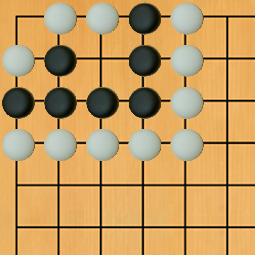
\includegraphics[scale=0.30]{figures/experiments/ko1.png}
    \caption{KO avant}
    \label{fig:button}
        
    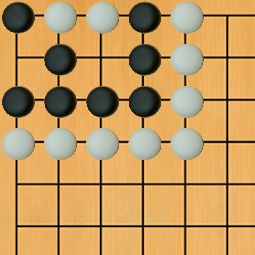
\includegraphics[scale=0.30]{figures/experiments/ko2.png}
    \caption{KO après}
    \label{fig:button}
    \end{figure}
    Un KO retourne vide après un seul coup et une pierre ne peut pas se poser sur un KO de la même couleur sauf si il mange un groupe qui est composé par plus d'une pierre.\\
    Le KO devient, plutôt qu'un algorithme, une intégration de l'algorithme de l'élimination des groupes.\\
                
    \section{Algorithme de définition des gobans fils d'un noeud}
    Pour chaque noeud de l'arbre on calcule tout les coups possibles du joueur et pour chaque coup on créé un goban. On aura de cette manière les gobans fils qui serons créé successivement à la base de ces premiers.\\
    Le nombre de gobans créés sera intuitivement le nombre d'états vides dans le goban de référence.
    Dans l'algorithme il y a les fonctions suivantes:\\
    \begin{itemize}
    \item \textbf{jouer(goban,pierre)}:
    contrôle si par rapport aux règles du jeu on peut poser la pierre dans le goban.\\
    Si le coup est possible alors l'appliquer et renvoyer vraie, sinon faux.
    \item \textbf{ajoute(e,t)}:
    Ajoute l'élément e en queue du tableau t.
    \item \textbf{rechercheGroupes(e,t)}:
    Ajoute l'élément e en queue du tableau t.
    \item \textbf{ajoute(e,t)}:
    Ajoute l'élément e en queue du tableau t.
    \end{itemize}
    
    
    \subsection{Algorithme du suicide}
    Le suicide est un coup avec lequel un joueur peut tuer un ou plusieurs groupe de sa propriété. Ce type de coup est illégal dans le jeu de go, il faudra donc que le programme détecte si un coup du joueur est un suicide ou pas. Pour cela on a créé l'algorithme suivant qui suit les étape suivantes :\\
        \begin{itemize}
            \item Vérifier si l'endroit où on va poser la pierre a des libertés afin de déterminer si c'est un suicide ou pas.
            \item Exécuter le coup sur un deuxième goban virtuel et lancer sur ce dernier la recherche de nouveaux groupes et l'élimination des groupes de l'adversaire relatif à la couleur de la pierre.
            \item Vérifier si le coup a tué un groupe adverse, indiquant alors que c'est pas un suicide.
            \item Enfin lancer sur le goban virtuel l'élimination des groupes de la même couleur que la pierre, puis vérifier si il tue un de ses groupes, prouvant alors le suicide.
        \end{itemize}
        Dans cet algorithme il y a 4 fonctions appelées qui auront les objectifs suivants:\\
        \begin{enumerate}
            \item \textbf{GroupesNoir(Goban)}: Soit une instance de la structure Goban passée en paramètre la fonction renvoie alors ses groupes noirs.
            \item \textbf{GroupesBlanc(Goban)}: Soit une instance de la structure Goban passée en paramètre la fonction renvoie alors ses groupes blancs.
            \item \textbf{PosePierreDansGoban(Pierre,Goban)}: Soit  une pierre et un goban la fonction pose la pierre sur le goban aux coordonnées stockées dans la variable pierre en vérifiant que l'endroit dans le goban soit vide.
            \item \textbf{EliminerGroupes(pierre, goban)}:Soit une pierre et un goban la fonction élimine les groupes sans libertés dans goban avec la même couleur que la pierre. 
            \item \textbf{EliminerGroupesAdversaire(pierre, goban)}:Soit une pierre et un goban la fonction élimine alors les groupes sans libertés dans goban avec la couleur opposée à la pierre initiale. 
        \end{enumerate}
        Il est important de préciser que la fonction de calcule des libertés d'une pierre sera nécessaire aussi.
    
    \begin{algorithme}
    \caption{Est-Suicide?}
    \textbf{Données :}
    \Type{Gob}{Goban},
    \Type{Pierre}{Etat};\\
    \textbf{Résultat :} Renvoie vrai si Pierre cause un suicide dans le Gob, renvoie faux sinon.\\
    \textbf{Variables :}   
    \Type{GroupesAVérifier}{Groupe[]},
    \Type{GroupesAdversaire}{Groupe[]},
    \Type{GroupesAdversaireAprès}{Groupe[]};\\
    \textbf{Début :}\\
     \If{taille(libertés(Pierre)) > 0}{ \textbf{renvoyer} faux}
     goban2 $\leftarrow$ goban\\
     \IfThenElse{Couleur(Pierre) = BLANC}{ GroupesAdversaire $\leftarrow$ groupesNoir(goban2)}{GroupesAdversaire $\leftarrow$ groupesBlanc(goban2)}
     JouerPierreDansGoban(Pierre, goban2)\\
     RechercheGroupes(goban2)\\
     EliminerGroupesAdversaire(Pierre, goban)\\
     \IfThenElse{Couleur(Pierre) = BLANC}{ 
     GroupesAdversaireAprès $\leftarrow$ groupesNoir(goban2)\\
     GroupesAVérifier $\leftarrow$ groupesBlanc(goban2)}
     {GroupesAdversaireAprès $\leftarrow$ groupesBlanc(goban2)\\
     GroupesAVérifier $\leftarrow$ groupesNoir(goban2)}
     \IfThenElse{taille(GroupesAdversaireAprès) < taille(GroupesAdversaire)}
     {\textbf{renvoyer} faux}{
     EliminerGroupes(Pierre, goban)\\
     \If{(Pierre = BLANC et taille(GroupesAVérifier) \neq taille(groupesBlanc(goban2))}{\textbf{renvoyer} vraie}
     \If{(Pierre = NOIR et taille(GroupesAVérifier) \neq taille(groupesNoir(goban2))}{\textbf{renvoyer} vraie}}
     {\textbf{renvoyer} faux}
\end{algorithme}
